\documentclass{article}

\usepackage{amsmath}
\usepackage{physics}
\usepackage{tikz, tikz-3dplot, pgfplots}
\usepackage{microtype}
\usepackage[letterpaper]{geometry}
\usepackage{float}

\pgfplotsset{compat=newest}

\newcommand{\dt}{\mathrm{d}t}
\newcommand{\x}{\mathrm{x}}
\newcommand{\y}{\mathrm{y}}
\newcommand{\z}{\mathrm{z}}
\newcommand{\vel}{\mathrm{v}}
\newcommand{\ddt}[1]{\frac{\mathrm{d}#1}{\dt}}
\newcommand{\dydt}{\frac{\mathrm{d}y}{\dt}}

\title{Newton's Law}
\date{2/6/2023}
\author{Laith}

\begin{document}
\maketitle

\section{Laws:}

\subsection*{First Law:}
    If an object is not experiencing the effect of any 
    force, then it will either remain stationary \textbf{or}
    keep moving with constant \underline{velocity}.

\subsection*{Second Law:}
    If force $\va{F}$ is acting on an object with 
    mass $m$, then the acceleration $\va{a}$ is given by:
    \[\va{F}=m\va{a}\]

\begin{figure}[H]
    \begin{tikzpicture}
        \draw (0, 0) -- (15, 0);

        \draw[thick] (1, 0) -- (1, 2);
        \draw[thick] (1.5, 0) -- (1.5, 1.5);
        \draw[thick] (4.5, 0) -- (4.5, 1.5);
        \draw[thick] (1.5, 1.5) -- (4.5, 1.5);
        \draw[thick] (1, 0) -- (1.5, 0);
        \draw[thick] (4.5, 0) -- (5, 0);
        \draw[thick] (5, 0) -- (5, 2);
        \draw[thick] (1, 2) -- (5, 2);
        \draw (2, 2) -- (2, 3);
        \draw (4, 2) -- (4, 3);
        \draw (2, 3) -- (4, 3);

        \draw[blue, stealth-stealth] (2.5, 0) node[below] {$Mg$} -- (2.5, 4) node[above] {$F_{\mathrm{table}}$};

        \node at (3, 2.5) {$M$};
    \end{tikzpicture} 
\end{figure}

Since the book is not moving, the net forces (sum of the forces) 
should equal 0 N. Since the forces are vectors, the forces must act 
in opposite directions in order for them to cancel out. Like you 
can see in the above figure, the force $F_\mathrm{table}$ of the table acts upwards, 
which is opposite of the force $m_g$ of gravity which is acting 
downwards. 

Mathematically, this would look like:
\[\sum F_{net} = F_\mathrm{table}+Mg = 0\,\mathrm{N}\]
Generally speaking, \textbf{a net force of 0 N means all 
components of force are 0}.

We can use free-body diagrams to model forces:
\begin{figure}[H]
    \begin{tikzpicture}
        \draw[<->] (0, -3) -- (0, 3) node[above] {$y$};
        \draw[<->] (-3, 0) -- (3, 0) node[right] {$x$};
    \end{tikzpicture}
\end{figure}

\section{Example Problem}

\begin{figure}[H]
   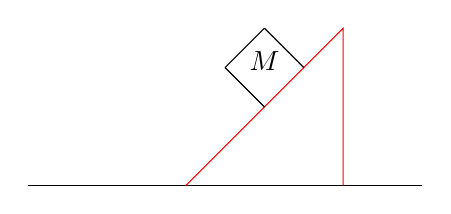
\begin{tikzpicture}
        \draw (0, 0) -- (5, 0);

        \draw[red] (2, 0) -- (4, 2) -- (4, 0);
        \draw (3.5, 1.5) -- (3, 2);
        \draw (3, 1) -- (2.5, 1.5);
        \draw (2.5, 1.5) -- (3, 2) node[below, yshift=-5] {$M$};
        
   \end{tikzpicture} 
\end{figure}

We can draw a free-body diagram to model the forces acting on the box with mass $M$:
\begin{figure}[H]
   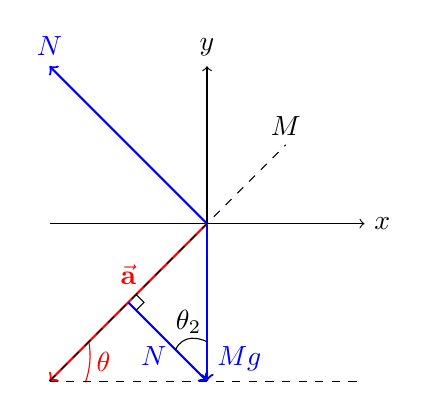
\begin{tikzpicture}
    \draw[->] (-2, 0) -- (2, 0) node[right] {$x$};
    \draw[->] (0, -2) -- (0, 2) node[above] {$y$};

    \draw[thick, blue, ->] (0, 0) -- (-2, 2) node[above] {$N$};
    \draw[thick, blue, ->] (0, 0) -- (0, -2) node[above right] {$Mg$};
    \draw[thick, red, ->] (0, 0) -- (-2, -2) node[midway, yshift=10] {$\va{a}$};
    \draw[thick, blue, ->] (-1, -1) -- (0, -2) node[midway, xshift = -5, yshift=-5] {$N$};
    \draw (-0.9, -0.9) -- (-0.8, -1) -- (-0.9, -1.1);
    \draw (0, -1.5) .. controls (-0.1, -1.45) and (-0.3, -1.4) .. (-0.4, -1.6) node[midway, yshift=6, xshift=-1] {$\theta_2$};
    \draw[red] (-1.5, -1.5) arc (10:-20:1) node[midway, xshift=5] {$\theta$};
    \draw[dashed] (-2, -2) -- (2, -2);
    \draw[dashed] (-2, -2) -- (1, 1) node[above] {$M$};
   \end{tikzpicture}
\end{figure}

\noindent Using the formula $\va{F}=M\va{a}$, we can determine the formulas for the 
$x$ and $y$ components of the net force. 

For the $x$ component, we need to look at the angle $\theta_2$ formed between the 
normal force vector $N$ and gravity vector $Mg$. We can see 
that the vectors form a triangle, which allows us to use the trigonmetric 
functions to setup an equation in which we can solve for $x$.
\[ \cos(\theta) = \frac{Mg}{x}\]

\noindent If the box starts from rest, how long does it take 
for it to come distance $l=1$ m down the incline?

% You are standing distance $d=2\mathrm{m}$ from your neighbor wall.
% The window is at height $h=1\mathrm{m}$ from the ground. You can 
% kick the ball such that it starts moving with speed $v=1\mathrm{m/s}$.
% With what angle with horizon should you kick the ball so that
% it hits the window?

\end{document}